


\documentclass[conference]{IEEEtran}




\usepackage{acronym}

\usepackage{array}
\usepackage{multirow}
\usepackage{epsfig}
\usepackage{xspace}
\usepackage{url}
%\usepackage[dvips]{color}
\usepackage{subfigure}
\usepackage{pgf}
\usepackage{pgfplots,pgfplotstable} %for plotting results
\usepgfplotslibrary{units}
\usepackage{amsmath}
\usepackage{amsfonts,amssymb}
\usepackage{mathrsfs}
\usepackage{filecontents}
\usepackage{tikz} % for drawing
\usetikzlibrary{arrows,shapes,fit,automata,positioning,decorations,calc} % for drawing
\usetikzlibrary{spy,backgrounds}
\usepackage{algorithmic, algorithm}
\newcounter{lemmas}
\newtheorem{lemma}{Lemma}
%\newcounter{proofs}
%\newtheorem{proof}{Proof}
\newcounter{theorems}
\newtheorem{theorem}{Theorem}


%\newtheorem*{proof*}{Theorem}
%\newtheorem*{proof}{Proof}



\newcounter{definitions}
\newtheorem{definition}{Definition}


\newcommand{\ignore}[1]{{}}
\newcommand{\ourTool}{Piha\xspace}
\newcommand{\iSignal}{\tau} %internal signal for HA
\newcommand{\inSignal}[1]{#1~} %input signal for HA
\newcommand{\outSignal}[1]{#1~} %output signal from HA

\newcolumntype{L}[1]{>{\raggedright\let\newline\\\arraybackslash\hspace{0pt}}m{#1}}
\newcolumntype{C}[1]{>{\centering\let\newline\\\arraybackslash\hspace{0pt}}m{#1}}
\newcolumntype{R}[1]{>{\raggedleft\let\newline\\\arraybackslash\hspace{0pt}}m{#1}}
  %Macros/#defs for the paper
\begin{document}
\acrodef{AP}{Action Potential}
\acrodef{ERP}{Effective Refractive Period}
\acrodef{CPS}{Cyber-physical Systems}
\acrodef{DSP}{Digital Signal Processor}
\acrodef{DTTS}{Discrete Time Transition System}
\acrodef{DHA}{Deterministic Hybrid Automata}
\acrodef{EA}{Evolutionary Algorithm}
\acrodef{HA}{Hybrid Automata}
\acrodef{ILP}{Integer Linear Programming}
\acrodef{MCU}{Microcontroller Unit}
\acrodef{ODE}{Ordinary Differential Equation}
\acrodef{PoC}{Plant-on-a-Chip}
\acrodef{RRP}{Relative Refractive Period}
\acrodef{RP}{Resting Period}
\acrodef{SHA}{Synchronous Hybrid Automata}
\acrodef{SWA}{Synchronous Witness Automata}
\acrodef{UP}{Upstroke}
\acrodef{WHA}{Well-formed Hybrid Automata}
\acrodef{WCET}{Worst-Case Execution Time}
\acrodef{FSM}{Finite State Machine}


\acrodef{NHC}{Network of Heart Cells}
\acrodef{WH}{Water Heating System}
\acrodef{MTG}{Multiple Train Gate control}
\acrodef{TSN}{Thermostat Network}
\acrodef{NP}{Nuclear Plant control}
 		%acronyms
	
\title{Modular code generation for emulating the electrical conduction system of the  human heart 
\ignore{Modular Code Generation from Hybrid Automata for Plant Emulation} }

\author{
	%blind review
	%\IEEEauthorblockN{Nathan Allen, Sidharta Andalam, Partha Roop and Avinash Malik}
	%\IEEEauthorblockA{Department of Electrical and Computer Engineering \\
	%	University of Auckland, New Zealand\\
	%	Email: \{nall426, sand080, p.roop, avinash.malik\}@aucklanduni.ac.nz
	%}
}





\maketitle





\begin{abstract}
  We study the problem of modular code generation for emulating the
  electrical conduction system of the heart, which is essential for the
  validation of implantable devices such as pacemakers. In order to
  develop high fidelity models, it is essential to consider the
  operation of hundreds, if not millions of conduction elements, called
  \emph{nodes} of the heart. Published results so far, however, have
  considered a maximum of 33~nodes, modelled as \acf{HIOA}. The
  behaviour of this model is captured using the well known commercial
  tool \simulink. The proposed approach is limiting due to the lack of
  model fidelity %as well as the lack of modelling the re-entrant nature
  of the conduction system.

  In this paper, we have developed a radically new approach to tackle
  the aforementioned drawbacks. We first develop a semantic preserving
  modular compilation approach for a network of \ac{HIOA}, by proposing
  to translate them to a network of \acp{FSM}. We then demonstrate that
  a delayed synchronous composition of the cardiac nodes enables modular
  code generation that is both semantic preserving and efficient. In
  addition to the above example, we have developed several examples from
  other domains to compare \simulink and the developed tool called
  \textit{Piha}. The results show that we are able to generate code that
  is on an average 54\% smaller in binary size while executing 9.8~times
  faster, on average, compared to \simulink.  We have also compared the
  scalability of the proposed approach relative to \simulink to prove
  its relative superiority.

  \ignore{Real-time emulation of a plant is often desirable to
    facilitate the testing of controllers under realistic conditions.
    Plants which exhibit continuous dynamics can be well modelled
    through the use of \acf{HIOA}, and so code generation from \ac{HIOA}
    that is suitable for real-time emulation is desirable.  In the case
    of plants which are modelled by a network of \acp{HIOA}, such code
    generation must be able to emulate the entire overall system through
    parallel composition.

    In this paper, we propose a new tool (named \ourTool) for the
    modular code generation from \ac{HIOA} that is amenable to use in
    both the real-time emulation or simulation of plants.  We illustrate
    the suitability of this approach through the running example of a
    human heart, where real-time emulation is desired for the
    verification of cardiac pacemakers.  We compare the proposed
    approach to \simulink, a tool commonly used in the modelling of
    plants, to show that we are able to generate code that is on average
    54\% smaller while executing 9.8 times faster.  We finish by showing
    the scalability of our approach in order to illustrate its potential
    in allowing real-time emulation of complex \ac{HIOA} networks.}
\end{abstract}


%%% Local Variables:
%%% mode: latex
%%% TeX-master: "../DATE2016_codegen"
%%% End:


\section{Introduction}

Pacemakers are safety-critical \acp{CPS} that control the pacing of a
heart for providing therapy for bradycardia -- abnormally slow pacing of
the heart. Such devices must operate in a fail-safe manner all the
time. However, between 1990-2000, close to 200,000 pacemakers have been
recalled due to software related
failures~\cite{alemzadeh13}. Considering this, there is a need for the
development of better processes for validation and certification of such
devices. We propose the well known, and widely used, engineering
technique of \emph{emulation}~\cite{patel2015survey} to tackle this
problem. Emulation, also known as hardware-in-the-loop simulation, is
used to validate controllers (such as motor controllers) by running them
in closed-loop with the actual plant (e.g., the synchronous motor).
However, for emulation of pacemakers, the use of the actual plant
(i.e. animal / human organs) is limiting. Hence, there is a need for the
development of high-fidelity heart models that can provide the required
real-time response to facilitate emulation. Bioengineering heart
models~\cite{Trayanova2014} provide excellent model fidelity at the
expense of computation time as the simulation of a single heart beat may
take several hours. Hence, such models are not suitable for emulation.

Recently, timed automata~\cite{zhihao12} based heart models have been
developed primarily for model checking. These models abstract the
continuous dynamics and hence, are unsuitable for emulation. In contrast
to this, \acf{HIOA}~\cite{alur2015book, raskin05} is used for modelling
the forward conduction system of the heart using 33 nodes
in~\cite{chen14} \footnote{Authors express their gratitude to the research 
	group of Prof. Marta Kwiatkowska for sharing their \simulink
	 heart model reported in~\cite{chen14}, 
	 which was foundational in developing the proposed models in this paper}. 
This work is the starting point for real-time
emulation by demonstrating that \simulink can be used for closed-loop
verification of pacemakers. However, this work has limited model
fidelity and the limitations of the tool \simulink are inherited by the
developed approach. \simulink has semantic limitations, as the semantics
of composition is unclear. Moreover, there is no
direct correspondence between the \simulink model and the \ac{HIOA}
models. Finally, \simulink generated code has scalability issues when 
generating large networks, as we will show.

% We develop an approach by combining node models (which are extensions
% to the models developed by~\cite{chen14}) with \emph{path models} (in
% timed automata) to accurately model the conduction delay between
% nodes. We are, thus, able to model the re-entrant behaviour of the
% heart.

 For modular code generation, we
have developed an approach based on the well known synchronous
languages~\cite{benveniste03}. % We formalise a subset of \ac{HIOA} called
% Synchronous Hybrid Input Output Automata \ac{SHIOA}.
Using the concept of delayed synchronous composition~\cite{SlLanguage},
we are then able to produce modular code for each node separately. The
generated code is both smaller and has faster execution times. In addition,
the generated code accurately captures the specification in \ac{HIOA},
similar in spirit to Ptolemy~\cite{ptolemaeus2014system} and
Z\'{e}lus~\cite{bourke13zelus}. However, unlike these approaches, the
presented approach does not depend upon dynamic numerical solvers, which
are not ideal for the \textit{emulation} of the heart.

\ignore{One reason that these malfunctions arise is due to the lack of
  proper validation. Unlike the ideas of hardware-in-the-loop testing,
  also known as \emph {emulation}~\cite{patel2015survey}, it is not
  possible to test on an actual heart. Further, unlike the hardware
  which is almost identical during mass production, each individual
  heart is different. Thus there is a need to develop a virtual heart
  that is tailored to an individual person and achieve personalised
  healthcare~\cite{Trayanova2014}. This idea can be extended to a
  network of human organs, resulting in a virtual human.

  Typically these biological models are developed by biomedical
  engineers. They mimic the heart's working at the molecular
  level~\cite{Trayanova2014}. To simulate one heart beat takes several
  hours, if not days. These models are very computationally intensive
  and are not suitable for real-time emulation, which is required for
  closed-loop testing of time-critical controllers such as cardiac
  pacemakers. Further, the models are very complex and hence are not
  amenable for formal verification. Thus, there is a need to develop
  abstract models by computer systems engineers that (1) \emph{capture
    the behaviour} of the heart (plant) from a pacemaker's
  (controller's) point of view, (2) \emph{allows for real-time
    emulation} of the heart such that it is possible for closed-loop
  simulation and (3) \emph{are amenable for formal verification} of
  functional and timing properties.

  The continuous dynamics of a plant (e.g. heart) and the discrete
  behaviour of a controller (e.g. pacemaker) result in so called hybrid
  systems. These are often formally described using
  \acf{HIOA}~\cite{alur2015principles,raskin05,chen201487}. However,
  these are non-deterministic and are problematic for generating
  constructive models. A more abstract deterministic model will enable
  us to develop constructive/synthesizable models~\cite{Lee2014}. Also,
  it is easier to draw trusted conclusions from simulations of
  deterministic models. Based on the well-known synchronous
  approach~\cite{benveniste03}, we present a deterministic semantics for
  \ac{HIOA} and show constructive models in this paper.

  Traditional \ac{CPS} design uses commercial tools such as \simulink
  for plant simulation and emulation. However, such designs do not
  preserve formal semantics of the models and are more verbose to
  describe. Academic tools for code generation from \ac{HIOA} models
  such as Ptolemy~\cite{ptolemaeus2014system} and
  Z\'{e}lus~\cite{bourke13zelus}. While these tools preserve the formal
  semantics, their reliance on dynamic numerical solvers makes them
  unsuitable for real-time emulation of plants. Such tools are capable
  of expressing the full non-deterministic nature of \acp{HIOA} rather
  than the deterministic subset described here.}

An overview of the proposed modular compilation approach is presented in
Figure~\ref{fig:overview}. It has two steps: (1) given a network of
\acp{HIOA}, step 1 generates a semantic preserving \ac{FSM}
representation of each \ac{HIOA} in the network. (2) Given a network of
such \acp{FSM}, step 2 then composes them using the synchronous parallel
operator ($||$) enabling generation of efficient `C'-code. Step 1 is
presented in Section~\ref{sec:codeGen}. Step 2 is presented in
Section~\ref{sec:composition}.


\begin{figure}[bthp]
  \centering \scalebox{0.7}{ % Define block styles
\tikzstyle{fileS} = [rectangle, draw, fill=red!20, 
text width=4em, text centered, minimum height=3em]
\tikzstyle{process} = [rectangle, draw, fill=blue!15, 
text width=9em, text centered, rounded corners, minimum height=4em]
\tikzstyle{line} = [draw, -latex', ultra thick]


\begin{tikzpicture}
% Place nodes

%-----------------------------------------------------------------------
\node [fileS,fill=red!10] (HA1) {$HIOA_1$ ($Def.~\ref{def:ha}$)};
\node[right of = HA1, node distance = 1.3cm](PAR){\Large $\dots$};
\node [fileS,,fill=red!10,right of = PAR, node distance = 1.3cm] (HA2) 
	{$HIOA_2$ ($Def.~\ref{def:ha}$)};	
%\node[below of = PAR, node distance=1.3cm, text width=3.7cm, text centered]
%	(TNHA){Network of HA};
%\node[draw, thick, inner sep=0.3cm, fit=(HA1) (HA2)] (NHA) {};

\node[draw, dashed, inner sep=0.3cm,
	label={[label distance=0cm]90:Section~\ref{sec:HA}}, 
	fit= (HA1) (HA2)] (S1) {};
%-----------------------------------------------------------------------


%\node [process, below  of = PAR, node distance = 2.2cm] (GSHA) {Generate FSM (step~1, Sec~\ref{sec:shaGeneration})};

%-----------------------------------------------------------------------
\node [fileS, below of = HA1, fill=red!20, node distance = 3.3cm] 
(FSM1) {$FSM_1$ ($Def.~\ref{def:ha}$)};
\node[right of = FSM1, node distance = 1.3cm](PAR){\Large $\dots$};
\node [fileS,,fill=red!20,right of = PAR, node distance = 1.3cm] (FSM2) 
{$FSM_2$ ($Def.~\ref{def:ha}$)};	

\node[draw, dashed, inner sep=0.3cm,
label={[label distance=0cm]90:Section~\ref{sec:codeGen}}, 
fit= (FSM1) (FSM2)] (S2) {};

%-----------------------------------------------------------------------
\node [fileS,,fill=blue!20, text width=8em, below of = PAR, node distance = 3.3cm] (PC) 
{$FSM_1 || FSM_2$ };
\node[ dashed, inner sep=0.1cm,
label={[label distance=0cm]90:Section~\ref{sec:composition}}, 
fit= (PC)] (S3) {};


%\node[draw, dashed, inner sep=0.2cm,
%	label={[label distance=0cm]60:Section~\ref{sec:SHA}}, 
%	fit= (GFSM)(CC)] (S3) {};

%--------------------------------------------------------------------------------
%edges
\draw [line] (HA1.south) -- (FSM1) node[midway, left]
{Step~1:  Code generation};
\draw [line] (HA2.south) -- (FSM2);
\draw [line] (FSM1) -- (FSM1|-PC.north) node[midway, left]
{Step~2:  Parallel composition};
\draw [line] (FSM2) -- (FSM2|-PC.north);
%\draw [line] (NSHA) -- (NSHA-|GFSM.west);
%\draw [line] (GFSM) -- (GFSM|-CC.south);

\end{tikzpicture}     }
  \caption{Overview of the proposed modular code generation
    approach \label{fig:overview}}
\end{figure}

\begin{figure*}[hbpt]
  \centering {
	\centering
	\subfigure[\label{fig:heart} Diagram of the heart. Reproduced 
	from~\cite{zhihao12}]{
       \framebox[0.31\textwidth]{
				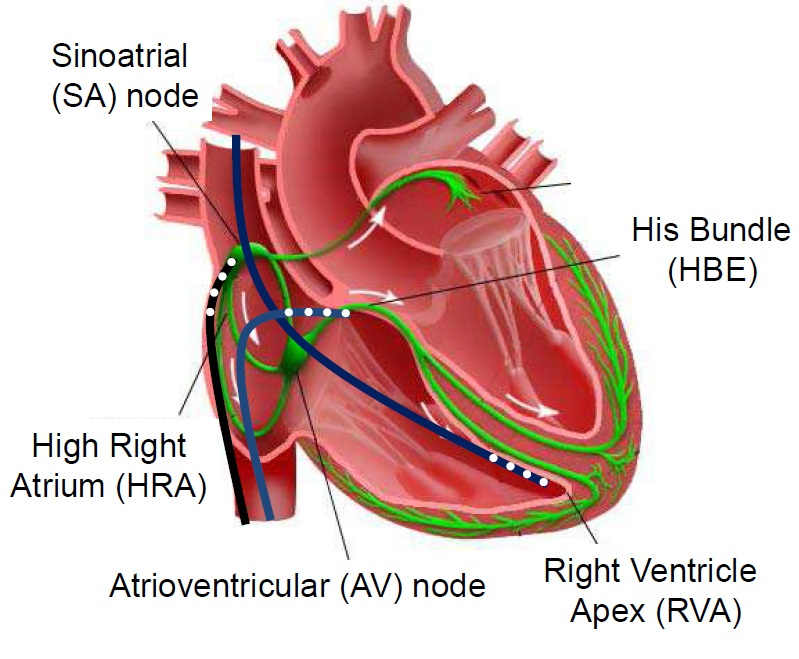
\includegraphics[width=0.262\linewidth]{figures/heart}
		} %framebox
	}
	\subfigure[The four stages of an \acf{AP}]{
		\framebox[0.31\textwidth]{
			\begin{tikzpicture}[transform shape, xscale=0.6, yscale=0.6]
\begin{axis}
[ xlabel={Time (ms)},
ylabel={Potential ({mV})},
axis y line = left,
axis x line = bottom,
xmin=0,   xmax=300,
ymin=0,   ymax=150,
ytick={0, 30, 44.5, 50, 100, 131.1, 150},
yticklabels={0, $v_R$, $v_T$, 50, 100, $v_O$, 150},
extra tick style={grid=major}
]
\addplot[color=blue!90,
mark=.,
mark size=2,
smooth,
const plot
]
table [x=t, y=v, col sep=comma] {./figures/actionPotentialData.csv};

\addplot[color=black!90,
dashed,
mark=.,
mark size=2
] coordinates {
	(0,30)
	(240,30)
};

\addplot[color=black!90,
dashed,
mark=.,
mark size=2
] coordinates {
	(0,44.5)
	(50,44.5)
};

\addplot[color=black!90,
dashed,
mark=.,
mark size=2
] coordinates {
	(0,131.1)
	(50,131.1)
};

\end{axis}

\tikzstyle{every state}=[rectangle, text centered, draw=none,text=black, draw,line width=0.3mm]

\node[state, shift={(0.2, -1.5)}, fill=green!20, inner xsep=0.0cm, minimum width=0.6cm] {RP};
\node[state, shift={(0.85, -1.5)}, fill=yellow!20, minimum width=0.5cm] {ST};
\node[state, shift={(3.00, -1.5)}, fill=red!20, minimum width=2.8cm] {ERP};
\node[state, shift={(1.50, -1.5)}, fill=blue!20, minimum width=0.5cm] {UP};
\node[state, shift={(5.15, -1.5)}, fill=green!20, minimum width=1.5cm] {RRP};
\node[state, shift={(6.40, -1.5)}, fill=green!20, minimum width=1cm] {RP};

\end{tikzpicture}
			\label{fig:actionPotential}
		}
	}
	\subfigure[An abstracted model of the conduction system]{ 
          \framebox[0.31\textwidth]{
          	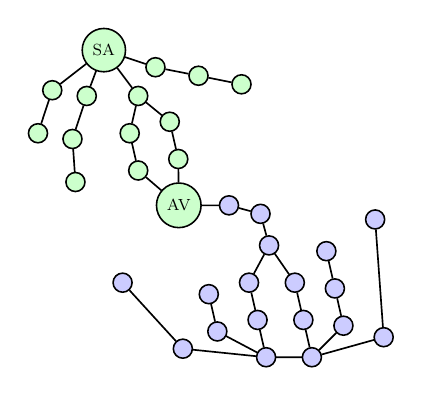
\begin{tikzpicture}[->,>=stealth',semithick,scale=0.73, transform shape]

\tikzstyle{every state}=[fill=blue!20,circle,minimum size=0.1cm]

\tikzset{
	atrialCell/.style={
		fill=green!20,
		circle,
		minimum size=0.1cm,
		draw,
		line width=0.2mm
	}
}

\tikzset{
	ventricularCell/.style={
		fill=blue!20,
		circle,
		minimum size=0.1cm,
		draw,
		line width=0.2mm
	}
}

\tikzset{
	autorhythmicCell/.style={
		fill=yellow!20,
		circle,
		minimum size=0.1cm,
		draw,
		line width=0.2mm
	}
}

\draw node[atrialCell](SA) {\footnotesize SA};

\node[atrialCell](CT) [below left=0.3cm and 0.5cm of SA] {};
\node[atrialCell](CT1) [below left=0.5cm and 0cm of CT] {};

\node[atrialCell](BB) [below right=-0.1cm and 0.5cm of SA] {};
\node[atrialCell](LA) [below right=-0.1cm and 0.5cm of BB] {};
\node[atrialCell](LA1) [below right=-0.1cm and 0.5cm of LA] {};

\node[atrialCell](RA) [below left=0.4cm and -0.1cm of SA] {};
\node[atrialCell](RA1) [below left=0.5cm and 0cm of RA] {};
\node[atrialCell](CS) [below left=0.5cm and -0.3cm of RA1] {};

\node[atrialCell](OS) [below right=0.4cm and 0.2cm of SA] {};
\node[atrialCell](Fast) [below left=0.4cm and -0.1cm of OS] {};
\node[atrialCell](Fast1) [below right=0.4cm and -0.1cm of Fast] {};
\node[atrialCell](Slow) [below right=0.2cm and 0.3cm of OS] {};
\node[atrialCell](Slow1) [below right=0.4cm and -0.1cm of Slow] {};
\node[atrialCell](AV) [below right=0.2cm and 0.3cm of Fast1] {\footnotesize AV};

\node[ventricularCell](His) [right=0.3cm of AV] {};
\node[ventricularCell](His1) [below right=-0.1cm and 0.3cm of His] {};
\node[ventricularCell](His2) [below right=0.3cm and -0.1cm of His1] {};

\node[ventricularCell](RBB) [below left=0.4cm and 0.1cm of His2] {};
\node[ventricularCell](RBB1) [below right=0.4cm and -0.1cm of RBB] {};
\node[ventricularCell](RVA) [below right=0.4cm and -0.1cm of RBB1] {};

\node[ventricularCell](LBB) [below right=0.4cm and 0.2cm of His2] {};
\node[ventricularCell](LBB1) [below right=0.4cm and -0.1cm of LBB] {};
\node[ventricularCell](LVA) [below right=0.4cm and -0.1cm of LBB1] {};

\node[ventricularCell](LVS) [above right=0.3cm and 0.3cm of LVA] {};
\node[ventricularCell](LVS1) [above left=0.4cm and -0.1cm of LVS] {};
\node[ventricularCell](CSLV) [above left=0.4cm and -0.1cm of LVS1] {};

\node[ventricularCell](LV) [above right=0.1cm and 1.0cm of LVA] {};
\node[ventricularCell](LV1) [above left=1.8cm and -0.1cm of LV] {};

\node[ventricularCell](RVS) [above left=0.2cm and 0.6cm of RVA] {};
\node[ventricularCell](RVS1) [above left=0.4cm and -0.1cm of RVS] {};

\node[ventricularCell](RV) [above left=-0.1cm and 1.2cm of RVA] {};
\node[ventricularCell](RV1) [above left=0.9cm and 0.8cm of RV] {};

\path[-] (SA) edge (BB);
\path[-] (BB) edge (LA);
\path[-] (LA) edge (LA1);

\path[-] (SA) edge (CT);
\path[-] (CT) edge (CT1);

\path[-] (SA) edge (RA);
\path[-] (RA) edge (RA1);
\path[-] (RA1) edge (CS);

\path[-] (SA) edge (OS);
\path[-] (OS) edge (Fast);
\path[-] (Fast) edge (Fast1);
\path[-] (OS) edge (Slow);
\path[-] (Slow) edge (Slow1);
\path[-] (Fast1) edge (AV);
\path[-] (Slow1) edge (AV);

\path[-] (AV) edge (His);
\path[-] (His) edge (His1);
\path[-] (His1) edge (His2);
\path[-] (His2) edge (RBB);
\path[-] (RBB) edge (RBB1);
\path[-] (RBB1) edge (RVA);
\path[-] (His2) edge (LBB);
\path[-] (LBB) edge (LBB1);
\path[-] (LBB1) edge (LVA);
\path[-] (RVA) edge (LVA);

\path[-] (RVA) edge (RVS);
\path[-] (RVS) edge (RVS1);

\path[-] (RVA) edge (RV);
\path[-] (RV) edge (RV1);

\path[-] (LVA) edge (LVS);
\path[-] (LVS) edge (LVS1);
\path[-] (LVS1) edge (CSLV);

\path[-] (LVA) edge (LV);
\path[-] (LV) edge (LV1);

\end{tikzpicture}
          	\label{fig:heartNetwork} 
	  } %framebox
	}

}
  \caption{Electrical conduction systems of the heart}
  \label{fig:heartOverview}
\end{figure*}

\textbf{Contributions} of the paper are:  %{\color{red} [AVINASH. I do
%  not agree with this contribution at all, it should be removed] we
%  propose a new definition for \acf{HIOA} (see Section~\ref{sec:HA}) to
%  capture the electrical conduction system of the heart.} 
  (1) We have
developed a \emph{modular code generation} approach, for the first time
for \ac{HIOA} models (Section~\ref{sec:codeGen}), which is also semantic
preserving. The proposed approach performs code generation using a new
synchronous semantics~\cite{benveniste03} of \ac{HIOA}. More
importantly, the developed semantics is not restrictive,
unlike~\cite{alur2003generating, kim2003modular} and does not interact
with dynamic numerical solvers unlike~\cite{ptolemaeus2014system,
  bourke13zelus}. (2) We \emph{quantitatively evaluate} the efficacy of
the proposed approach relative \simulink
(Section~\ref{sec:benchmarking}) to demonstrate the scalability of the
approach relative to the best known model in published
literature~\cite{chen14}. Our experiments show that code generation is
feasible for thousands of nodes of the heart, unlike the 33-node
published model. % We have also modelled a much more realistic human heart
% as the modelled system can mimic its re-entrant behaviour.




%%% Local Variables:
%%% mode: latex
%%% TeX-master: "../DATE2016_codegen"
%%% End:

\section{Background on the Heart }
\begin{figure*}[htbp]
	\centering
	{
	\centering
	\subfigure[\label{fig:heart} Diagram of the heart. Reproduced 
	from~\cite{zhihao12}]{
       \framebox[0.31\textwidth]{
				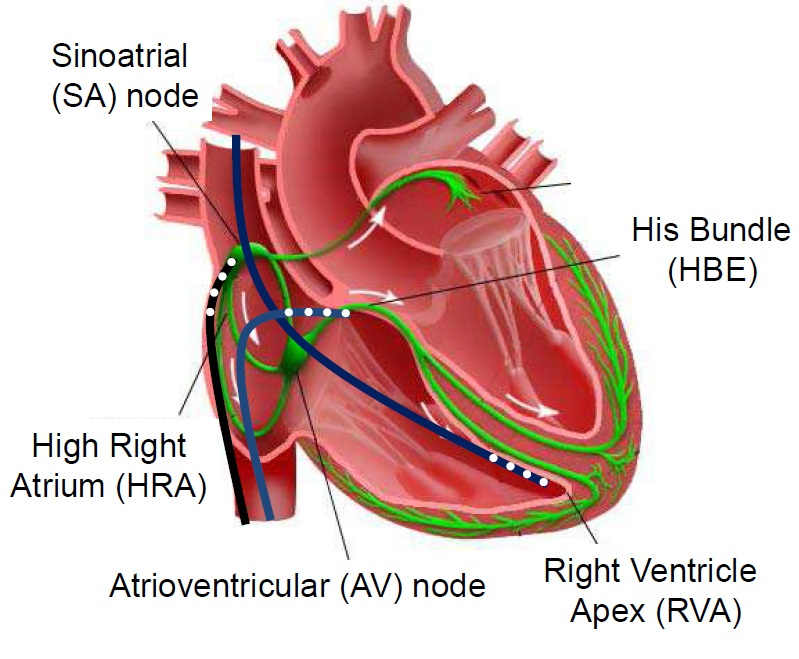
\includegraphics[width=0.262\linewidth]{figures/heart}
		} %framebox
	}
	\subfigure[The four stages of an \acf{AP}]{
		\framebox[0.31\textwidth]{
			\begin{tikzpicture}[transform shape, xscale=0.6, yscale=0.6]
\begin{axis}
[ xlabel={Time (ms)},
ylabel={Potential ({mV})},
axis y line = left,
axis x line = bottom,
xmin=0,   xmax=300,
ymin=0,   ymax=150,
ytick={0, 30, 44.5, 50, 100, 131.1, 150},
yticklabels={0, $v_R$, $v_T$, 50, 100, $v_O$, 150},
extra tick style={grid=major}
]
\addplot[color=blue!90,
mark=.,
mark size=2,
smooth,
const plot
]
table [x=t, y=v, col sep=comma] {./figures/actionPotentialData.csv};

\addplot[color=black!90,
dashed,
mark=.,
mark size=2
] coordinates {
	(0,30)
	(240,30)
};

\addplot[color=black!90,
dashed,
mark=.,
mark size=2
] coordinates {
	(0,44.5)
	(50,44.5)
};

\addplot[color=black!90,
dashed,
mark=.,
mark size=2
] coordinates {
	(0,131.1)
	(50,131.1)
};

\end{axis}

\tikzstyle{every state}=[rectangle, text centered, draw=none,text=black, draw,line width=0.3mm]

\node[state, shift={(0.2, -1.5)}, fill=green!20, inner xsep=0.0cm, minimum width=0.6cm] {RP};
\node[state, shift={(0.85, -1.5)}, fill=yellow!20, minimum width=0.5cm] {ST};
\node[state, shift={(3.00, -1.5)}, fill=red!20, minimum width=2.8cm] {ERP};
\node[state, shift={(1.50, -1.5)}, fill=blue!20, minimum width=0.5cm] {UP};
\node[state, shift={(5.15, -1.5)}, fill=green!20, minimum width=1.5cm] {RRP};
\node[state, shift={(6.40, -1.5)}, fill=green!20, minimum width=1cm] {RP};

\end{tikzpicture}
			\label{fig:actionPotential}
		}
	}
	\subfigure[An abstracted model of the conduction system]{ 
          \framebox[0.31\textwidth]{
          	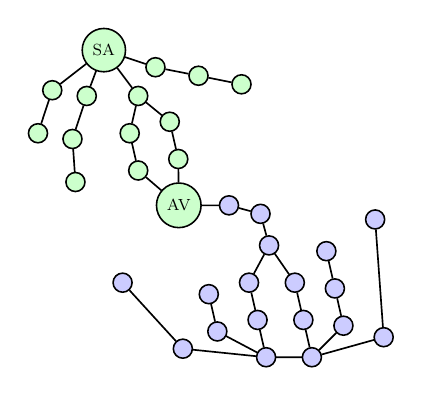
\begin{tikzpicture}[->,>=stealth',semithick,scale=0.73, transform shape]

\tikzstyle{every state}=[fill=blue!20,circle,minimum size=0.1cm]

\tikzset{
	atrialCell/.style={
		fill=green!20,
		circle,
		minimum size=0.1cm,
		draw,
		line width=0.2mm
	}
}

\tikzset{
	ventricularCell/.style={
		fill=blue!20,
		circle,
		minimum size=0.1cm,
		draw,
		line width=0.2mm
	}
}

\tikzset{
	autorhythmicCell/.style={
		fill=yellow!20,
		circle,
		minimum size=0.1cm,
		draw,
		line width=0.2mm
	}
}

\draw node[atrialCell](SA) {\footnotesize SA};

\node[atrialCell](CT) [below left=0.3cm and 0.5cm of SA] {};
\node[atrialCell](CT1) [below left=0.5cm and 0cm of CT] {};

\node[atrialCell](BB) [below right=-0.1cm and 0.5cm of SA] {};
\node[atrialCell](LA) [below right=-0.1cm and 0.5cm of BB] {};
\node[atrialCell](LA1) [below right=-0.1cm and 0.5cm of LA] {};

\node[atrialCell](RA) [below left=0.4cm and -0.1cm of SA] {};
\node[atrialCell](RA1) [below left=0.5cm and 0cm of RA] {};
\node[atrialCell](CS) [below left=0.5cm and -0.3cm of RA1] {};

\node[atrialCell](OS) [below right=0.4cm and 0.2cm of SA] {};
\node[atrialCell](Fast) [below left=0.4cm and -0.1cm of OS] {};
\node[atrialCell](Fast1) [below right=0.4cm and -0.1cm of Fast] {};
\node[atrialCell](Slow) [below right=0.2cm and 0.3cm of OS] {};
\node[atrialCell](Slow1) [below right=0.4cm and -0.1cm of Slow] {};
\node[atrialCell](AV) [below right=0.2cm and 0.3cm of Fast1] {\footnotesize AV};

\node[ventricularCell](His) [right=0.3cm of AV] {};
\node[ventricularCell](His1) [below right=-0.1cm and 0.3cm of His] {};
\node[ventricularCell](His2) [below right=0.3cm and -0.1cm of His1] {};

\node[ventricularCell](RBB) [below left=0.4cm and 0.1cm of His2] {};
\node[ventricularCell](RBB1) [below right=0.4cm and -0.1cm of RBB] {};
\node[ventricularCell](RVA) [below right=0.4cm and -0.1cm of RBB1] {};

\node[ventricularCell](LBB) [below right=0.4cm and 0.2cm of His2] {};
\node[ventricularCell](LBB1) [below right=0.4cm and -0.1cm of LBB] {};
\node[ventricularCell](LVA) [below right=0.4cm and -0.1cm of LBB1] {};

\node[ventricularCell](LVS) [above right=0.3cm and 0.3cm of LVA] {};
\node[ventricularCell](LVS1) [above left=0.4cm and -0.1cm of LVS] {};
\node[ventricularCell](CSLV) [above left=0.4cm and -0.1cm of LVS1] {};

\node[ventricularCell](LV) [above right=0.1cm and 1.0cm of LVA] {};
\node[ventricularCell](LV1) [above left=1.8cm and -0.1cm of LV] {};

\node[ventricularCell](RVS) [above left=0.2cm and 0.6cm of RVA] {};
\node[ventricularCell](RVS1) [above left=0.4cm and -0.1cm of RVS] {};

\node[ventricularCell](RV) [above left=-0.1cm and 1.2cm of RVA] {};
\node[ventricularCell](RV1) [above left=0.9cm and 0.8cm of RV] {};

\path[-] (SA) edge (BB);
\path[-] (BB) edge (LA);
\path[-] (LA) edge (LA1);

\path[-] (SA) edge (CT);
\path[-] (CT) edge (CT1);

\path[-] (SA) edge (RA);
\path[-] (RA) edge (RA1);
\path[-] (RA1) edge (CS);

\path[-] (SA) edge (OS);
\path[-] (OS) edge (Fast);
\path[-] (Fast) edge (Fast1);
\path[-] (OS) edge (Slow);
\path[-] (Slow) edge (Slow1);
\path[-] (Fast1) edge (AV);
\path[-] (Slow1) edge (AV);

\path[-] (AV) edge (His);
\path[-] (His) edge (His1);
\path[-] (His1) edge (His2);
\path[-] (His2) edge (RBB);
\path[-] (RBB) edge (RBB1);
\path[-] (RBB1) edge (RVA);
\path[-] (His2) edge (LBB);
\path[-] (LBB) edge (LBB1);
\path[-] (LBB1) edge (LVA);
\path[-] (RVA) edge (LVA);

\path[-] (RVA) edge (RVS);
\path[-] (RVS) edge (RVS1);

\path[-] (RVA) edge (RV);
\path[-] (RV) edge (RV1);

\path[-] (LVA) edge (LVS);
\path[-] (LVS) edge (LVS1);
\path[-] (LVS1) edge (CSLV);

\path[-] (LVA) edge (LV);
\path[-] (LV) edge (LV1);

\end{tikzpicture}
          	\label{fig:heartNetwork} 
	  } %framebox
	}

}
	\caption{Electrical conduction systems of the heart}
	\label{fig:heartOverview}
\end{figure*}

In this section, using Figure~\ref{fig:heartOverview} we 
describe the electrical conduction system of the heart.

\noindent \textbf{Heart.}
The human heart (see Figure~\ref{fig:heart})
 is an organ that pumps blood throughout the body.
It achieves this by regularly contracting and relaxing the muscles
which are orchestrated by a flow of electrical signals through the heart.
The signal is primarily generated automatically by the \ac{SA} node.
First, the signal travels through the left and right atria, contracting 
the muscles and pushing the blood into the ventricles.
 
Second, to ensure both ventricles are filled, 
the \ac{AV} node introduces critical delay 
in the conduction system.   
Finally, the electrical signal propagates through 
both ventricles. This contracts the muscles and pumps the blood out of the heart.


\noindent \textbf{\acf{AP}.} 
The propagation of electrical signals at a cellular level 
is described as a change in  voltage 
across the cell membrane due to ionic flow. Over a period of time, 
this change is known as an \acf{AP}~\cite{chen14} as shown in Figure~\ref{fig:actionPotential}. 
The \ac{AP} can be described in four stages.
\begin{enumerate}
	\item \acf{RP}: This is the steady state of the cell while awaiting 
					activation by an external stimulus.
	\item \acf{UP}: When activated by an external stimulus, 
					the cell depolarises (inward flow of positive ions) and 
					contracts the muscles. This depolarisation yields 
					a stimulus that activates neighbouring cells.
	\item \acf{ERP}: Once activated, the cell cannot be activated again 
					 due to the recovery process of the ionic channels. 
					 Any new stimulus will be blocked. 
	\item \acf{RRP}: During this period, the ionic channels are partially recovered
					 and the cell can be activated. However, the morphology
					 of the \ac{AP} will be shorter.
	
\end{enumerate}


\noindent \textbf{Abstract model.}
The human heart has over two trillion cells. For analytical purposes, a
model consisting of a network of $32$ nodes is presented in literature
and is used for testing off-the-shelf pacemakers~\cite{chen14,zhihao12}.
The abstracted electrical conduction system consisting  of 
nodes and paths is presented in Figure~\ref{fig:heartNetwork}.
The functionality of each node is described using \acf{HA} in Section~\ref{sec:HA}. The path model describes the 
conduction delay of the electrical signal.
Later in Section~\ref{sec:codeGen}, we use the abstract network model 
to illustrate our modular code generation.

 

\section{Hybrid Automata}
\label{sec:HA}

\acf{HIOA} is ideal for describing \ac{CPS}. It is very expressive,
non-deterministic and has been successfully used for capturing the
behaviour of a plant in control systems. In this section, we use the
\ac{HIOA} in Figure~\ref{fig:heartCellHA}, which captures the \ac{AP} in
Figure~\ref{fig:actionPotential} as a running example to provide a
formal definition and an informal description of the semantics of
\ac{HIOA}.

\subsection{Example of \acf{HIOA} }

\begin{figure}
  \centering 
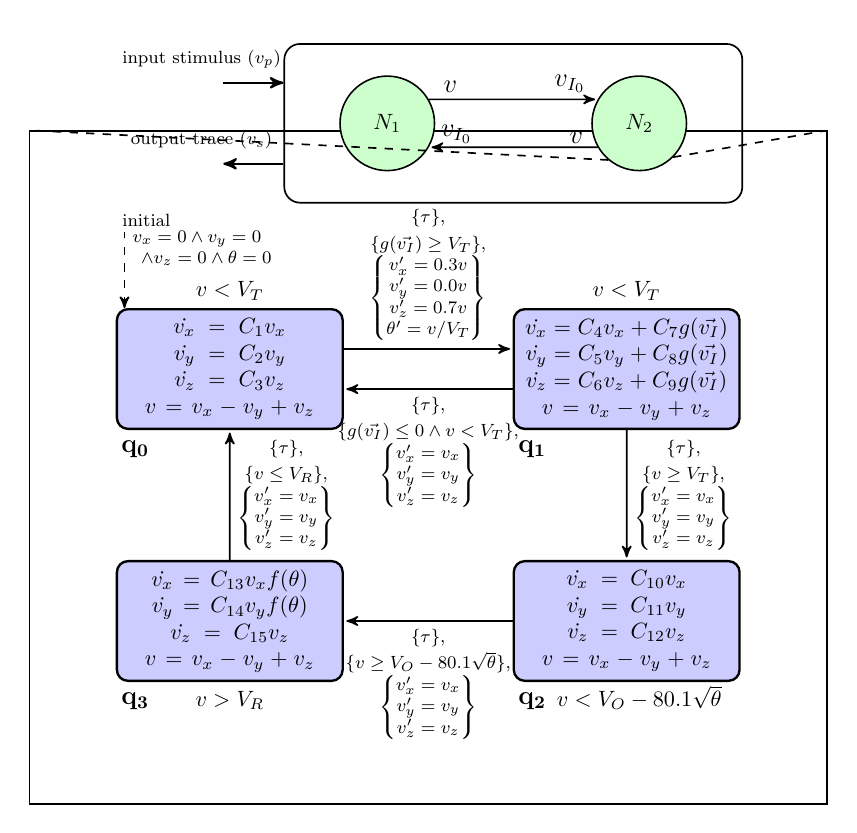
\begin{tikzpicture}[->,>=stealth',shorten >=1pt,auto,
node distance=4cm,
semithick,scale=0.8, transform shape]
\tikzstyle{every state}=[rectangle,rounded corners,
 minimum height = 1.9cm, text width=3.35cm, text centered, fill=blue!20,draw=none,text=black, draw,line width=0.3mm]
 \tikzset{
 	atrialCell/.style={
 		fill=green!20,
 		circle,
 		minimum size=1.5cm,
 		draw,
 		line width=0.2mm
 	}
 }
 


\node[state, 
label={[shift={(0,0)}]$v < V_T$}, 
label={[shift={(-1.5,-2.5)}]\large $ \mathbf{q_0}$ }]
(Q0)  {$\dot{v_x}=C_1 v_x$ \\ $\dot{v_y}=C_2 v_y$ \\ $\dot{v_z}=C_3 v_z$ \\ $v=v_x - v_y + v_z$};

%entry
\path[<-, dashed] (Q0.150) edge node[below, align=left, shift={(1.15,1)}] {
	\footnotesize initial \\
	\footnotesize $\begin{matrix}
		v_{x}=0 \wedge v_{y}=0 \\
		\quad \wedge v_{z}=0 \wedge \theta=0
	\end{matrix}$
} ++(0cm,1.25cm);




\node[state, 
label={[shift={(0,0)}]$v < V_T$}, 
label={[shift={(-1.5,-2.5)}]\large $\mathbf{q_1}$   }]
(Q1) [node distance=6.3cm, right of=Q0] {$\dot{v_x}=C_4 v_x + C_7 g(\vec{v_{I}})$ \\ $\dot{v_y}=C_5 v_y + C_8 g(\vec{v_{I}})$ \\ $\dot{v_z}=C_6 v_z + C_9 g(\vec{v_{I}})$ \\ $v=v_x - v_y + v_z$};

\node[state, 
label={[shift={(0.2,-2.5)}]$v < V_O - 80.1 \sqrt{\theta}$}, 
label={[shift={(-1.5,-2.5)}]\large $\mathbf{q_2}$  }] 
(Q2) [below of=Q1] {$\dot{v_x}=C_{10} v_x$ \\ $\dot{v_y}=C_{11} v_y$ \\ $\dot{v_z}=C_{12} v_z$ \\ $v=v_x - v_y + v_z$};

\node[state, 
label={[shift={(0,-2.5)}]$v > V_R$}, 
label={[shift={(-1.5,-2.5)}]\large $\mathbf{q_3}$  }]
(Q3) [below of=Q0] {$\dot{v_x}=C_{13} v_x f(\theta)$ \\ $\dot{v_y}=C_{14} v_y f(\theta)$ \\ $\dot{v_z}=C_{15} v_z$ \\ $v=v_x - v_y + v_z$};

\path[->] (Q0.10) edge node[align=center] {
	\footnotesize $\{\tau\}$, \\
	\footnotesize $\{g(\vec{v_{I}}) \geq V_T\}$, \\
	\footnotesize $\left\{\begin{matrix} v^\prime_x = 0.3v \\ v^\prime_y = 0.0v \\ v^\prime_z = 0.7v \\ \theta^\prime = v / V_T \end{matrix}\right\}$
} (Q1.170);

\path[->] (Q1.190) edge node[align=center] {
	\footnotesize $\{\tau\}$, \\
	\footnotesize $\{g(\vec{v_{I}}) \leq 0 \wedge v < V_T$\}, \\
	\footnotesize $\left\{\begin{matrix} v^\prime_x = v_x \\ v^\prime_y = v_y \\ v^\prime_z = v_z \end{matrix}\right\}$
} (Q0.350);

\path[->] (Q1) edge node[align=center] {
	\footnotesize $\{\tau\}$, \\
	\footnotesize $\{v \geq V_T\}$, \\
	\footnotesize $\left\{\begin{matrix} v^\prime_x = v_x \\ v^\prime_y = v_y \\ v^\prime_z = v_z \end{matrix}\right\}$
} (Q2);

\path[->] (Q2) edge node[align=center] {
	\footnotesize $\{\tau\}$, \\
	\footnotesize $\{v \geq V_O - 80.1\sqrt{\theta}\}$, \\
	\footnotesize $\left\{\begin{matrix} v^\prime_x = v_x \\ v^\prime_y = v_y \\ v^\prime_z = v_z \end{matrix}\right\}$
} (Q3);

\path[->] (Q3) edge node[align=center, shift={(1.8,0)}] {
	\footnotesize $\{\tau\}$, \\
	\footnotesize $\{v \leq V_R\}$, \\
	\footnotesize $\left\{\begin{matrix} v^\prime_x = v_x \\ v^\prime_y = v_y \\ v^\prime_z = v_z \end{matrix}\right\}$
} (Q0);


\node[ draw,   inner xsep=1.1cm, inner ysep=1.9cm, shift={(0, 0.35)},
label={[label distance=0cm]60:~}, 
fit= (Q0)(Q2)] (BOX) {};

%--------------------------- nodes on top ------------
\node[atrialCell, above of = Q0, xshift=2.5cm, node distance = 3.9cm,
label={[shift={(1,-0.4)}]\large $v$ },
label={[shift={(1.1,-1.2)}]\large $v_{I_{0}}$ }]
(AN1){$N_1$};
\node[atrialCell, right of = AN1, node distance = 4cm,
label={[shift={(-1.1,-0.4)}]\large $v_{I_{0}}$ },
label={[shift={(-1,-1.2)}]\large $v$ }] 
(AN2){$N_2$};
\draw[->](AN1.30) -- (AN2.150);
\draw[->](AN2.210) -- (AN1.-30);


\draw[-,dashed](AN2.-45) -- (BOX.north east);
\draw[-,dashed](AN2.230) -- (BOX.north west);

%---------------- pacemaker I/O ------------
\node[ draw,  rounded corners=2mm, inner xsep=0.7cm,inner ysep=0.4cm,
label={[label distance=0cm]60:~}, 
fit= (AN1)(AN2)] (BOX2) {};

\draw[<-, thick](BOX2.170) -- node[above, shift={(-0.8,0.1)}] {\footnotesize input stimulus ($v_p$)} ++(-1cm,0cm);

\draw[->, thick](BOX2.190) -- node[above, shift={(-0.8,0.1)}] {\footnotesize output trace ($v_s$)} ++(-1cm,0cm);


\end{tikzpicture}


%%% Local Variables:
%%% mode: latex
%%% TeX-master: "../DATE2016_codegen"
%%% End:

  \caption{Top of the figure shows the interaction between two heart nodes 
    ($N_1$ and $N_2$). Each node is defined as a \acf{HIOA} 
    \label{fig:heartCellHA}}
\end{figure}

The heart node \ac{HIOA}, shown in Figure~\ref{fig:heartCellHA}, captures the
behaviour of the four stages of \ac{AP} shown in
Figure~\ref{fig:actionPotential}. Each stage of the \ac{AP} is captured
using locations in the \ac{HIOA}. The \ac{AP} of every node, in
the heart, evolves over time, this evolution of the \ac{AP} is captured
with three \acfp{ODE} evolving three individual variables: $v_{x}$,
$v_{y}$, and $v_{z}$, respectively. The overall voltage of the \ac{AP}
is then aggregated into a single variable $v$ as defined
in~\cite{YeESG08}. The aggregated \ac{AP} voltage $v$ of each node
effects its neighbouring nodes and vice-versa. This effect of the
neighbouring voltages is captured in the \ac{HIOA} via function
$g(\vec{v_{I}})$, where $\vec{v_{I}}$ represents the \emph{vector} of
voltages. Finally, the dynamic response of the action potential to
secondary excitation is captured by the variable~$\theta$.

For the first stage (\ac{RP}), the continuous dynamics are captured in
location $\mathbf{q_0}$. \acfp{ODE}, for example \mbox{$\dot{v_{x}} = 
C_{1}v_{x}$}, capture the continuous evolution of components of $v$ ($v_{x}$, 
$v_{y}$, $v_{z}$) when control resides in location $\mathbf{q_{0}}$ 
while the location invariant $v < V_{T}$ holds.  Once the external
stimulus, $g(\vec{v_{I}})$, crosses some threshold $V_{T}$, indicated by
the predicate \mbox{$g(\vec{v_{I}} \geq V_{T})$} on the edge connecting
locations $\mathbf{q_{0}}$ and $\mathbf{q_{1}}$, the \ac{HIOA}
transitions to location $\mathbf{q_{1}}$
\textit{instantaneously}. During this transition, the variables (e.g,
$v^{\prime}_{x}$) are updated. These updated values of the variables are
used as initial conditions from which the variables evolve further via
the \acp{ODE} in the target location.

Once the voltage of the node ($v$) exceeds the threshold voltage
$V_{T}$, it begins its \ac{ERP} phase (captured by location
$\mathbf{q_2}$). The final location, $\mathbf{q_3}$, represents the
\ac{RRP} stage. The constants $C_1$ through to $C_{15}$, configure the
morphology of the \ac{AP}. Furthermore, constants $V_T$, $V_O$, and
$V_R$ determine the height of the \ac{AP} and transitions between
locations of the \ac{HIOA} to further capture the morphology.

% The voltage of any node in the heart effects its neighboring nodes and
% vice-versa. Hence, a means to communicate the voltages of the node to
% its neighbors is needed. We achieve this communication between nodes of
% the heart using the input and output variables and events available in
% the \ac{HIOA} framework. 


We formalise the \ac{HIOA} using Definition~\ref{def:ha}.

\begin{definition}
  % \label{def:1}
  A \acf{HIOA} \newline $\mathcal{H}$ =
  $\langle Loc, Edge, \Sigma_I, \Sigma_{EO}, \Sigma_{EI}, X_I, X_{EO},
  X_{EI}, \linebreak Init, Inv, Flow, Up, Jump\rangle$ where
  \begin{itemize}
  \item $Loc=\{l_1,..,l_n\}$ representing $n$ locations.
  \item $\Sigma_{E} = \Sigma_{EI} \cup \Sigma_{EO}$ is the set of
    external events. $\Sigma_{EI}$ and $\Sigma_{EO}$ are the set of
    external input and external output events,
    respectively. Furthermore,
    \mbox{$\Sigma_{EI} \cap \Sigma_{EO} = \emptyset$}.
  \item $\Sigma=\Sigma_{E} \cup \{\iSignal\}$ is set of event names
    comprising of external and the $true$ event, respectively.
  \item
    $Edge \subseteq Loc \times \mathcal{B}(\Sigma_{EI} \cup \{\tau\})
    \times 2^{\Sigma_{EO}} \times Loc$
    are the set of edges between locations.
  \item Three sets for the set of internal continuous variables, their
    rate of change and their updated values represented as follows:
    $X_I=\{x_1,.., x_m\}$, $\dot{X_I}=\{\dot{x_1},.., \dot{x_m}\}$, and
    $X_I'=\{x_{1}',.., x_{m}'\}$.
  \item The set of external continuous variables:
    \mbox{$X_E = X_{EI} \cup X_{EO}$}. Furthermore,
    \mbox{$X_{EI} \cap X_{EO} = \emptyset$}.
  \item $Init(l)$: Is a predicate whose free variables are from
    $X_{I}$. It specifies the possible valuations of these when the HIOA
    starts in $l$.
  \item $Inv(l)$: Is a predicate whose free variables are from
    \mbox{$X_I \cup X_{E}$} and it constrains these when the HIOA
    resides in $l$.
  \item $Flow(l)$: Is a predicate whose free variables are from
    $X_I \cup \dot{X_I}$ and it specifies the rate of change of these
    variables when the HIOA resides in $l$.
  \item $Up(l)$: Is a function that assigns to each variable in set
    $X_{EO}$ an algebraic expression involving the variables from \mbox{$X_{I} 
    \cup X_{EI}$}.
  \item $Jump(e)$: Is a function that assigns to the edge `$e$' a
    predicate whose free variables are from $X_I \cup X_I' \cup X_E$.
    This predicate specifies when the location switch using `$e$' is
    possible. It also specifies the updated values of the variables when
    this location switch happens.
  \end{itemize}
  \label{def:ha}
\end{definition}

For the \ac{HIOA} in Figure~\ref{fig:heartCellHA},
$Loc=\{q_{0},q_{1},q_{2},q_{3}\}$, $\Sigma_{EI} = \emptyset$,
$\Sigma_{EO}=\emptyset$, and
$\Sigma=\{\tau\}$. \mbox{$X_{I}=\{\theta,v_{x},v_{y},v_{z}\}$},
\mbox{$\dot{X_{I}}=\{\dot{\theta},\dot{v_{x}},\dot{v_{y}},\dot{v_{z}}\}$},
\mbox{$X^{\prime}_{I}=\{\theta',{v'_{x}},{v'_{y}},\dot{v'_{z}}\}$}.
$X_{EI}=\{v_{i}| \forall v_{i} \in \vec{v_{I}}\}$. $X_{EO}=\{v\}$. An
example of initial predicate is: 
\mbox{$Init(l): (v_{x}=0 \wedge v_{y}=0 \wedge v_{z}=0 \wedge \theta=0)$}. An
example edge connecting locations $q_{0}$ and $q_{1}$ is represented
with the tuple: $(q_{0},\tau,\emptyset,q_{1})$. The example of invariant
($Inv$) predicate on location $q_{0}$ is: $v < V_{T}$. The $Jump$ condition on
the edge connecting locations $q_{0}$ and $q_{1}$ is enabled when the
predicate \mbox{$g(\vec{v_{I}} \geq V_{T})$} is true, and the updated
variables are as shown in Figure~\ref{fig:heartCellHA}. An example of
the $Up$ predicate is the function $v = v_{x} - v_{y} + v_{z}$ in all
locations in Figure~\ref{fig:heartCellHA}. Finally, the $Flow$ predicate
in location $q_{0}$ are the set of \acp{ODE}, in location
$\mathbf{q_{0}}$ in Figure~\ref{fig:heartCellHA}.

% \begin{definition}[Hybrid Automata]
%   \label{def:ha}
%   $HIOA = \langle Loc, X, \Sigma, Init, Inv, Flow, Jump \rangle$ where
%   %   Locations
%   $Loc=\{q_0,q_1,q_2,q_3\}$ is a set of locations.
%   $X=\{v,v_x,v_y,v_z,\theta\}$ is a set of continuous variables.
%   $\Sigma=\Sigma_I \cup \Sigma_O \cup \{\iSignal\}$ is a set of input,
%   output, and internal events.  $Init=\{(q_0,v): v < V_T\}$ is the
%   initial condition.  $Inv=\{(q_3,v): v > V_R\}$ is the invariant.
%   $Flow=\{(q_0,v_x): C_1 v_x\}$ specifies the continuous flow rate.
%   $Jump=\{(q_n, q_m): signal, cond, update\}$: describes the discrete
%   transition from $q_n$ and $q_m$ which is enabled when $signal$ is
%   present and the $cond$ evaluates to true, perfoms and $update$
%   during this transition.  Further, to remove non-determinism, we must
%   ensure that for all locations there does not exist more than one
%   active $Jump$ transition.
% \end{definition}

% {\color{red} Given $m$ number of \acp{HIOA} in a network. The network
% can be described as $HIOA_1 || \dots || HIOA_m$.}

% \section{\acf{SHIOA}}
% \label{sec:SHA}

% Every \ac{HIOA} is converted into a so called \ac{SHIOA}, where the
% ODEs in the flow predicates are replaced by their equivalent witness
% functions $Switness$. The witness function computes the evolution of
% the continuous variables using the forward Euler approach with a
% \emph{constant} step size. Before giving the formal definition of the
% \ac{SHIOA} and describing the compilation procedure, we present the
% procedure to convert each ODE into its equivalent witness function,
% this is the step 1 (c.f. Figure~\ref{fig:overview}) in our modular
% code generation framework.

% \renewcommand{\algorithmiccomment}[1]{// #1}
% \renewcommand{\algorithmicrequire}{\textbf{Input:}}
% \renewcommand{\algorithmicensure}{\textbf{Output:}}
% \begin{algorithm}[t!]
%   \begin{algorithmic}[1]
%     \REQUIRE Network of HIOA has \ENSURE Network of SHIOA shas
%     \FORALL{$ha \in has$} \label{alg:HAsToSHAs:allHAs}
%     \FORALL{$loc \in ha$} \label{alg:HAsToSHAs:allLocs}
%     \FORALL{$ode \in loc$} \label{alg:HAsToSHAs:allODEs} \STATE
%     $eq \leftarrow create\_euler(ode)$
%     \label{alg:HAsToSHAs:createEuler} \STATE $ode \leftarrow
%     eq$ \label{alg:HAsToSHAs:assignOde}
%     \ENDFOR
%     \ENDFOR
%     \ENDFOR
%     \RETURN this
%   \end{algorithmic}
%   \caption{The algorithm to generate a Network of \acp{SHIOA} from a
%   Network of \acp{HIOA}}
%   \label{alg:HAsToSHAs}
% \end{algorithm}

% The procedure for performing this conversion across the entire network
% of \acp{HIOA} to generate a network of \acp{SHIOA} is shown in
% Algorithm~\ref{alg:HAsToSHAs}. The algorithm needs to visit every
% \ac{HIOA} in the network, every location within each \ac{HIOA}, and
% every \ac{ODE} in each location (lines~\ref{alg:HAsToSHAs:allHAs} -
% \ref{alg:HAsToSHAs:allODEs}). For each of these \acp{ODE} the forward
% Euler equivalent is created in the same manner as described earlier
% (line~\ref{alg:HAsToSHAs:createEuler}). Each \ac{ODE} is eventually
% replaced (line~\ref{alg:HAsToSHAs:assignOde}) by its equivalent
% numerical solution in order to form the network of \acp{SHIOA}.

% \subsection{Definition of \acf{SHIOA}}
% \label{sec:defSHA}

% \begin{figure}
%   \centering 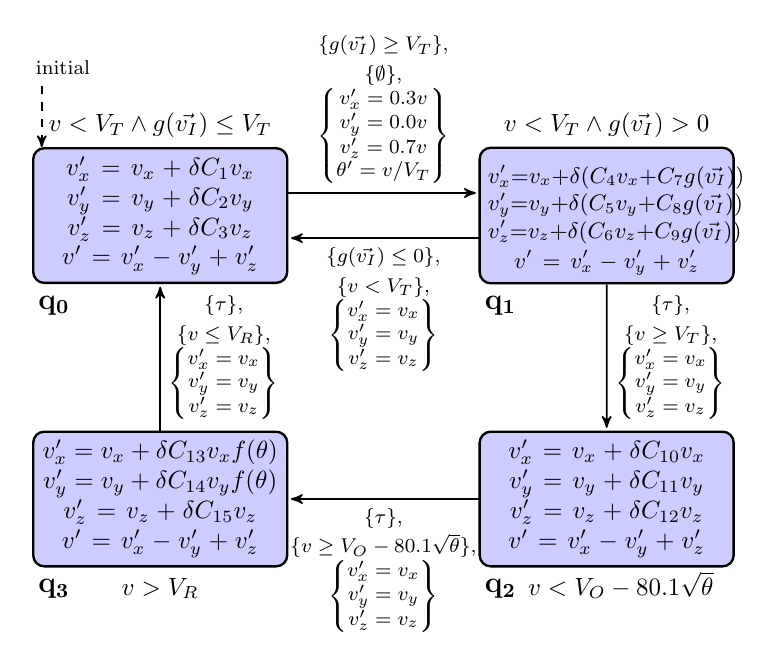
\begin{tikzpicture}[->,>=stealth',shorten >=1pt,auto,
node distance=4cm,
semithick,scale=0.9, transform shape]
\tikzstyle{every state}=[rectangle,rounded corners,
 minimum height = 1.9cm, text width=3.35cm, text centered, fill=blue!20,draw=none,text=black, draw,line width=0.3mm]

\node[state, 
label={[shift={(0,0)}]$v < V_T \wedge g(\vec{v_{I}}) \leq V_T$}, 
label={[shift={(-1.5,-2.5)}]\large $ \mathbf{q_0}$ }]
(Q0)  {$v^\prime_x = v_x + \delta C_{1} v_x$ \\ $v^\prime_y = v_y + \delta C_{2} v_y$ \\ $v^\prime_z = v_z + \delta C_{3} v_z$ \\ $v^\prime=v^\prime_x - v^\prime_y + v^\prime_z$};

%entry
\draw[<-, dashed](Q0.150) -- node[above, shift={(0.3,0.4)}] {\footnotesize initial} ++(0cm,1cm);




\node[state, 
label={[shift={(0,0)}]$v < V_T \wedge g(\vec{v_{I}}) > 0$}, 
label={[shift={(-1.5,-2.5)}]\large $\mathbf{q_1}$   }]
(Q1) [node distance=6.3cm, right of=Q0] {\small{ $v^\prime_x {=} v_x {+} \delta (C_{4} v_x {+} C_{7} g(\vec{v_{I}}))$ \\ $v^\prime_y {=} v_y {+} \delta (C_{5} v_y {+} C_{8} g(\vec{v_{I}}))$ \\ $v^\prime_z {=} v_z {+} \delta (C_{6} v_z {+} C_{9} g(\vec{v_{I}}))$ \\ $v^\prime=v^\prime_x - v^\prime_y + v^\prime_z$}};

\node[state, 
label={[shift={(0.2,-2.5)}]$v < V_O - 80.1 \sqrt{\theta}$}, 
label={[shift={(-1.5,-2.5)}]\large $\mathbf{q_2}$  }] 
(Q2) [below of=Q1] {$v^\prime_x = v_x + \delta C_{10} v_x$ \\ $v^\prime_y = v_y + \delta C_{11} v_y$ \\ $v^\prime_z = v_z + \delta C_{12} v_z$ \\ $v^\prime=v^\prime_x - v^\prime_y + v^\prime_z$};

\node[state, 
label={[shift={(0,-2.5)}]$v > V_R$}, 
label={[shift={(-1.5,-2.5)}]\large $\mathbf{q_3}$  }]
(Q3) [below of=Q0] {$v^\prime_x = v_x + \delta C_{13} v_x f(\theta)$ \\ $v^\prime_y = v_y + \delta C_{14} v_y f(\theta)$ \\ $v^\prime_z = v_z + \delta C_{15} v_z$ \\ $v^\prime=v^\prime_x - v^\prime_y + v^\prime_z$};

\path[->] (Q0.10) edge node[align=center] {
	\footnotesize $\{g(\vec{v_{I}}) \geq V_T\}$, \\
	\footnotesize $\{\emptyset\}$, \\
	\footnotesize $\left\{\begin{matrix} v^\prime_x = 0.3v \\ v^\prime_y = 0.0v \\ v^\prime_z = 0.7v \\ \theta^\prime = v / V_T \end{matrix}\right\}$
} (Q1.170);

\path[->] (Q1.190) edge node[align=center] {
	\footnotesize $\{g(\vec{v_{I}}) \leq 0\}$, \\
	\footnotesize $\{v < V_T\}$, \\
	\footnotesize $\left\{\begin{matrix} v^\prime_x = v_x \\ v^\prime_y = v_y \\ v^\prime_z = v_z \end{matrix}\right\}$
} (Q0.350);

\path[->] (Q1) edge node[align=center] {
	\footnotesize $\{\tau\}$, \\
	\footnotesize $\{v \geq V_T\}$, \\
	\footnotesize $\left\{\begin{matrix} v^\prime_x = v_x \\ v^\prime_y = v_y \\ v^\prime_z = v_z \end{matrix}\right\}$
} (Q2);

\path[->] (Q2) edge node[align=center] {
	\footnotesize $\{\tau\}$, \\
	\footnotesize $\{v \geq V_O - 80.1\sqrt{\theta}\}$, \\
	\footnotesize $\left\{\begin{matrix} v^\prime_x = v_x \\ v^\prime_y = v_y \\ v^\prime_z = v_z \end{matrix}\right\}$
} (Q3);

\path[->] (Q3) edge node[align=center, shift={(1.8,0)}] {
	\footnotesize $\{\tau\}$, \\
	\footnotesize $\{v \leq V_R\}$, \\
	\footnotesize $\left\{\begin{matrix} v^\prime_x = v_x \\ v^\prime_y = v_y \\ v^\prime_z = v_z \end{matrix}\right\}$
} (Q0);

\end{tikzpicture}
%   \caption{\acf{SHIOA} of a heart node \label{fig:heartCellSHA}}
% \end{figure}

% A \ac{SHIOA} is an abstraction of the corresponding \ac{HIOA}. It
% inherits all the components of a \ac{HIOA} except that the ODEs in the
% $Flow$ predicates are replaced by their individual witness functions
% $Switness$. The
% $Switness(l,\delta,\vec{v}_{l,X_{I}})=\vec{v}^{\prime}_{l,X_{I}}$,
% function returns the new values of continuous variables in location
% $l$ after one iteration of step size $\delta$ given the current
% valuation ($\vec{v}^{\prime}_{l,X_{I}}$) of continuous variables in
% $X_{I}$. We now formalise the \ac{SHIOA} using
% Definition~\ref{def:sha} and illustrate it using
% Figure~\ref{fig:heartCellSHA}.

% \begin{definition}
%   Given a well formed HIOA $\mathcal{H}$ =
%   $\langle Loc, Edge, \Sigma_I, \Sigma_{EO}, \Sigma_{EI}, X_I, X_{EO},
%   X_{EI}, \linebreak Init, Inv, Flow, Jump\rangle$
%   a SHIOA corresponding to this HIOA is $\mathcal{A}$ =
%   $\langle Loc, Edge, \Sigma_I, \Sigma_{EO}, \Sigma_{EI}, X_I,
%   X_{EO},\linebreak X_{EI}, Init, Inv, Witness, Jump, Step\rangle$
%%   where:
%   \begin{itemize}
%   \item $Step = \delta$ ($\delta \in \mathbb{R}^+$) is the duration of
%     the synchronous instant.
%   \item
%     $Switness: Loc \times \mathbb{R} \times \mathbb{R}^{\|X_{I}\|}
%     \rightarrow \mathbb{R}^{\|X_{I}\|}$:
%     is the Euler function(s) that returns the new values of all the
%     continuous variables for a given location $l$. It also takes as
%     input the time step $\delta$ and the current values of all
%     variables in set $X_{I}$.
%   \end{itemize}
%   \label{def:sha}
% \end{definition}

% {\color{red} Given $m$ number of \acp{SHIOA} in a network. The network
% can be described as $SHIOA_1 || \dots || SHIOA_m$.}

% \subsection{Deterministic semantics of \ac{SHIOA}}
% \label{sec:DTTS}
% Deterministic semantics of a \ac{SHIOA} is provided as a \acf{DTTS} in
% Definition~\ref{def:dtts}. We assume that all transitions of a
% \acf{DTTS} trigger relative to the ticks of the logical clock of the
% synchronous program.
% 
% \begin{definition}
%   The semantics of a \newline
%   $SHIOA = \langle Loc, \Sigma, Init, Inv, Switness, Jump, Step
%   \rangle$
%   is a $DTTS = \langle Q, Q^0, \Sigma, \rightarrow \rangle$ where
%   
%   \begin{itemize}
%   \item The state-space is $Q$, where any state is of the form
%     $(l, v, i, k)$ where $l$ is a location, $i$ is the initial
%     valuation of the variables when execution begins in the location
%     and $v$ is the valuation at the $k$-th instant.
%   \item $Q^0 \subseteq Q$ where every $q^0 \in Q^0$ is of the form
%     $(l, v^0, i, k)$ such that $v$ satisfies $Init(l)$.
%   \item Transitions are of two types:
%     \begin{itemize}
%     \item \emph{Inter-location transitions} that lead to a change in
%       location: These are of the form
%       $(l, v, i, k) \stackrel{\sigma} \rightarrow (l', v', i', 0)$ if
%       $(l, v, i, k) \in Q$, $(l', v', i', 0) \in Q$,
%       $e=(l \stackrel{\sigma} \rightarrow l') \in Edge$ and $(v, v')$
%       satisfy $Jump(e)$.
%     \item \emph{Intra-location transitions} made during the execution
%       in a given mode / location: These are of the form
%       $(l, v, i, k) \rightarrow (l, v', i, k+1)$ if
%       $(l, v, i, k) \in Q$, $(l, v', i, k+1) \in Q$, $(v, v')$ satisfy
%       $Inv(l)$, $Switness(l,k,\delta,i)=v$ and
%       $Switness(l,k+1,\delta,i)=v'$.
%     \end{itemize}
%     
%			\item Restriction: Inter-location transitions
%     always have \emph{higher} priority over {Intra-location
%     transitions}. This avoids the non-determinism.
%   \end{itemize}
%   \label{def:dtts}
% \end{definition}

% \subsection{Generation of a network of \ac{SHIOA}}
% \label{sec:shaGeneration}

% This section describes step $1$ of the compilation process from
% Figure~\ref{fig:overview}. This step involves converting all of the
% \acp{ODE} in each of the \acp{HIOA} into their forward Euler
% equivalent methods.

%%% Local Variables:
%%% mode: latex
%%% TeX-master: "../DATE2016_codegen"
%%% End:

\section{Modular code generation}
\label{sec:codeGen}

In this section we present our approach for modular code generation from
a network of \acp{HIOA} as it is implemented in our tool, called
\ourTool.  An overview of the solution is presented in 
Figure~\ref{fig:overview}. Firstly, we present how each \ac{ODE} is converted 
to its numerical equivalent in Section~\ref{sec:converting-odes-into} followed 
by code generation for a single \ac{HIOA} through the use of a Mealy \ac{FSM} 
in Section~\ref{sec:backendCodeGeneration}.

\subsection{Converting the \acp{ODE} into equivalent witness functions}
\label{sec:converting-odes-into}

Given the \ac{ODE} for $\dot{v_x}$ in state $\mathbf{q_0}$ of the heart
node \ac{HIOA} defined in Figure~\ref{fig:heartCellHA} (reproduced in
Equation~(\ref{eq:ode})), the forward Euler method computes the next
value of $v_{x}$ (denoted $v'_{x}$) at discrete time instants, separated
by the so called time step $\delta$
($\delta \in \mathbb{R}^{+}$). The witness function for $v_{x}$
implementing the forward Euler method is shown in
Equation~(\ref{eq:euler_equiv}). This witness function evolves the
variable $v_{x}$ until some invariant condition $Inv$ on the location
holds. For the current example, Equation~(\ref{eq:euler_equiv}) evolves
$v_{x}$ \emph{iteratively} until the invariant condition on location
$\mathbf{q_{0}}$ ($v < V_{T}$) holds.


\begin{equation}
  \dot{v_x} = C_{1} v_x
  \label{eq:ode}
\end{equation}

\begin{equation}
  v^\prime_x = v_x + \delta \times (C_{1} v_x)
  \label{eq:euler_equiv}
\end{equation}


This iterative evolution of the continuous variables at discrete points
in time is akin to transitions on a logical \emph{tick} of a
synchronous program~\cite{benveniste03}. A likeness that we will exploit when 
composing multiple \ac{HIOA} together in Section~\ref{sec:composition}.


\subsection{Backend code generation for a single \ac{HIOA}}
\label{sec:backendCodeGeneration}

\begin{figure}
  \centering
  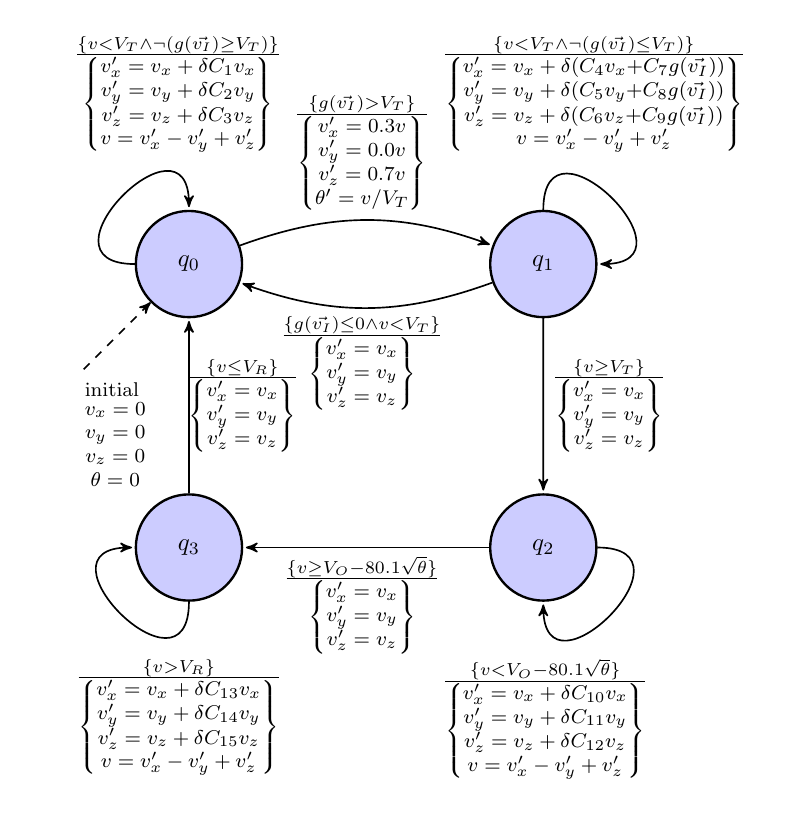
\begin{tikzpicture}[->,>=stealth',shorten >=1pt,auto,node distance=4cm,
semithick,scale=0.9, transform shape]
\tikzstyle{every state}=[circle,rounded corners,
minimum height = 1.2cm, text width=1.2cm, text
centered, fill=blue!20,draw=none,text=black,
draw,line width=0.3mm]

\node[state] (Q0)  { $q_0$ };

\path[<-, dashed] (Q0.225) edge node[below, align=left, shift={(0,-0.5)}] {
	\footnotesize initial \\
	\footnotesize $\begin{matrix}
		v_x = 0 \\
		v_y = 0 \\
		v_z = 0 \\
		\theta = 0
	\end{matrix}$
} ++(-1cm,-1cm);

\node[state]
(Q1) [node distance=5cm, right of=Q0] 	 {$q_1$};

\node[state] 
(Q2) [below of=Q1] 	 {$q_2$};

\node[state] 
(Q3) [below of=Q0] 	 { $q_3$};


%inter-location transitions
\path[->] (Q0.20) edge[out=20,in=160] node[align=center] {
  $\frac{\footnotesize \{g(\vec{v_{I}}) > V_T\}}
  {\footnotesize
  \left\{\begin{matrix} v^\prime_x = 0.3v \\ v^\prime_y = 0.0v \\
      v^\prime_z = 0.7v \\ \theta^\prime = v / V_T \end{matrix}\right\}}$
} (Q1.160);

\path[->] (Q1.200) edge[out=200,in=340] node[align=center] {
	$\frac{\footnotesize \{g(\vec{v_{I}}) \leq 0 \wedge v < V_T\}}
	{\footnotesize \left\{\begin{matrix} v^\prime_x = v_x \\ v^\prime_y = v_y \\ v^\prime_z = v_z \end{matrix}\right\}}$
} (Q0.340);

\path[->] (Q1) edge node[align=center] {
	$\frac{\footnotesize \{v \geq V_T\}}
	{\footnotesize \left\{\begin{matrix} v^\prime_x = v_x \\ v^\prime_y = v_y \\ v^\prime_z = v_z \end{matrix}\right\}}$
} (Q2);

\path[->] (Q2) edge node[align=center] {
	$\frac{\footnotesize \{v \geq V_O - 80.1\sqrt{\theta}\}}
	{\footnotesize \left\{\begin{matrix} v^\prime_x = v_x \\ v^\prime_y = v_y \\ v^\prime_z = v_z \end{matrix}\right\}}$
} (Q3);

\path[->] (Q3) edge node[align=center, shift={(1.8,0)}] {
	$\frac{\footnotesize \{v \leq V_R\}}
	{\footnotesize \left\{\begin{matrix} v^\prime_x = v_x \\ v^\prime_y = v_y \\ v^\prime_z = v_z \end{matrix}\right\}}$
} (Q0);

%intra-location transitions
\path[->] (Q0.180) edge[out=180,in=90,distance=1.5cm] node[align=center,
shift={(2.5,0.5)}] {
  $\frac{\footnotesize \{v < V_T \wedge \neg (g(\vec{v_{I}}) \geq V_T)\}}
  {\footnotesize \left\{\begin{matrix}
      v^\prime_x = v_x + \delta C_{1} v_x \\
      v^\prime_y = v_y + \delta C_{2} v_y \\
      v^\prime_z = v_z + \delta C_{3} v_z \\
      v=v^\prime_x - v^\prime_y + v^\prime_z
	\end{matrix}\right\}}$
} (Q0.90);

\path[->] (Q1.90) edge[out=90,in=0,distance=1.5cm] node[align=center,
shift={(-2.5,0.5)}] {
  $\frac{\footnotesize \{v < V_T \wedge \neg (g(\vec{v_{I}}) \leq V_T)\}}
  {\footnotesize \left\{\begin{matrix}
      v^\prime_x = v_x + \delta (C_{4} v_x {+} C_{7} g(\vec{v_{I}})) \\
      v^\prime_y = v_y + \delta (C_{5} v_y {+} C_{8} g(\vec{v_{I}})) \\
      v^\prime_z = v_z + \delta (C_{6} v_z {+} C_{9} g(\vec{v_{I}})) \\
      v=v^\prime_x - v^\prime_y + v^\prime_z
	\end{matrix}\right\}}$
} (Q1.0);

\path[->] (Q2.0) edge[out=0,in=-90,distance=1.5cm] node[align=center,
shift={(-2.5,-0.5)}] {
  $\frac{\footnotesize \{v < V_O - 80.1 \sqrt{\theta}\}}
  {\footnotesize \left\{\begin{matrix}
      v^\prime_x = v_x + \delta C_{10} v_x \\
      v^\prime_y = v_y + \delta C_{11} v_y \\
      v^\prime_z = v_z + \delta C_{12} v_z \\
      v=v^\prime_x - v^\prime_y + v^\prime_z
	\end{matrix}\right\}}$
} (Q2.-90);

\path[->] (Q3.-90) edge[out=-90,in=180,distance=1.5cm]
node[align=center, shift={(2.5,-0.5)}] {
  $\frac{\footnotesize \{v > V_R\}}
  {\footnotesize \left\{\begin{matrix}
      v^\prime_x = v_x + \delta C_{13} v_x \\
      v^\prime_y = v_y + \delta C_{14} v_y \\
      v^\prime_z = v_z + \delta C_{15} v_z \\
      v=v^\prime_x - v^\prime_y + v^\prime_z
	\end{matrix}\right\}}$
} (Q3.180);

\end{tikzpicture}


%%% Local Variables:
%%% mode: latex
%%% TeX-master: "../DATE2016_codegen"
%%% End:

  \caption{\acf{FSM} of a heart node \label{fig:heartCellFSM}. We ignore
    the $\tau$ event in the \ac{FSM}, because it always evaluates to $true$.}
\end{figure}

In order to facilitate code generation, each \ac{HIOA} is transformed into a 
simple Mealy \ac{FSM} (such as that shown in Figure~\ref{fig:heartCellFSM}) 
where each iteration of the program requires a transition be taken.  Each 
inter-location edge $e$ corresponds to a transition between the same two states 
with condition equal to its input events conjuncted with the conditions in 
$Jump(e)$, and output equal to its output events combined with the updates 
present in $Jump(e)$.

In order to replicate the continuous evolution of variables within locations we 
create self transitions on each state in $Loc$, where the invariant in $Inv$ 
becomes the condition of the transition, and the witness functions for each of 
the \acs{ODE} described in Section~\ref{sec:converting-odes-into} become the 
output of the transition. However, to ensure that the generated \ac{FSM} does 
not ignore any controller inputs the self transition of each state must be of 
the lowest priority.  This is accomplished by changing the condition to be 
conjuncted with the negation of the disjunction of all conditions of egress 
transitions from the state, i.e. $Inv(l) \wedge \neg (Cond(trans_{0}) \vee 
\dots \vee Cond(trans_{n})$.  For example, in state $\mathbf{q_0}$ the 
invariant $v < V_{T}$ will become a self transition with a condition of $v < 
V_{T} \wedge \neg (g(\vec{v_{I}}) \geq V_{T})$ in the generated \ac{FSM}.

The final corresponding \ac{FSM} for the \ac{HIOA} from 
Figure~\ref{fig:heartCellHA} is shown in Figure~\ref{fig:heartCellFSM}.

Each of these \acp{FSM} are then transformed into C code which contains an 
\emph{Initialisation Function} corresponding to the $Init$ of the \ac{FSM} as 
well as the setting of the initial state, and a \emph{Run Function} which, 
given an existing state $l$ and values for all variables $X$ and events 
$\Sigma$, performs a single transition and updates any variables or events that 
may have changed.

\section{Parallel Composition}
\label{sec:composition}

\subsection{Synchronous Parallel}
\label{sec:synchronousParallel}

%\begin{figure}
%  \centering
%  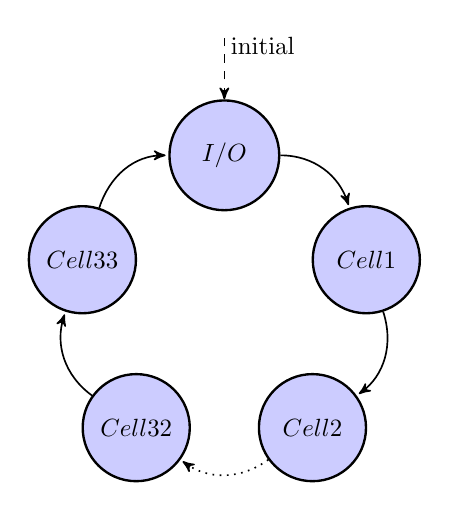
\begin{tikzpicture}[->,>=stealth',shorten >=1pt,auto,node distance=4cm,
semithick,scale=0.9, transform shape]
\tikzstyle{every state}=[circle,rounded corners,
minimum height = 1.2cm, text width=1.2cm, text
centered, fill=blue!20,draw=none,text=black,
draw,line width=0.3mm]

\node[state] (IO)  { $I/O$ };

\path[<-, dashed] (IO.90) edge node[above, align=center, shift={(0.6,0)}] {
	initial
} ++(0cm,1cm);

\node[state]
(Cell1) [below right=0.37cm and 0.9cm of IO] 	 {$Cell1$};

\node[state]
(Cell2) [below left=1.28cm and -0.33cm of Cell1] 	 {$Cell2$};

\node[state]
(Cell33) [below left=0.37cm and 0.9cm of IO] 	 {$Cell33$};

\node[state]
(Cell32) [below right=1.28cm and -0.33cm of Cell33] 	 {$Cell32$};


\path[->] (IO.0) edge[out=0,in=108] (Cell1.108);

\path[->] (Cell1.-72) edge[out=-72,in=36] (Cell2.36);

\path[->, dotted] (Cell2.-144) edge[out=-144,in=-36] (Cell32.-36);

\path[->] (Cell32.-216) edge[out=-216,in=-108] (Cell33.-108);

\path[->] (Cell33.-288) edge[out=-288,in=-180] (IO.-180);

\end{tikzpicture}
%  \caption{Synchronous composition of multiple heart
%    cells \label{fig:heartCellComposition}}
%\end{figure}

In order to compose each of the \acp{FSM} together, we take inspiration
from the concepts of Synchronous Languages such as SL~\cite{SlLanguage}.  The 
concept of Ticks and Reactions are carried over, whereby each \ac{FSM} performs 
only a single transition (``tick'') until all other \acp{FSM} have also 
completed a transition (``reaction'') and the process can repeat.  In order to
deal with data dependencies, we also implement the concept of \emph{pre}
whereby the value of all inputs to each \ac{FSM} are not updated with
new values until the end of each reaction.  This allows for the behaviour of 
the system to be agnostic to the scheduling order of the individual 
\acp{FSM}.  This concept also enables us to simplify the process of 
handling cyclic \acp{ODE} (an issue that other work such as 
\cite{kim2003modular} do not consider) by causing the dependencies to reference
previous, rather than current, values.

The implementation of this in \ourTool is done by creating a round-robin
scheduler which executes one tick of each \ac{FSM} (the \emph{Run Function} 
described in Section~\ref{sec:backendCodeGeneration}) in series, followed by an 
\emph{I/O Synchronisation Stage} at the end of each reaction.  Such I/O 
synchronisation deals with the emission of all outputs from the system, the 
intake of all inputs to the system, and the transfer of signals between 
\acp{FSM} in the network, the mapping of which is described in  
Section~\ref{sec:mapping}.  This process continues indefinitely to emulate the 
dynamics of the system.  In addition, when the system initially starts up it 
enters an \emph{Initialisation Stage} whereby the \emph{Initalisation Function} 
for each \ac{FSM} is run before continuing on to the round-robin loop mentioned 
above.

Due to the scheduling order agnosticism described earlier, this concept is 
amenable to further scheduling algorithms that need not be sequential in 
nature.  \ourTool can be extended to support parallel computation by executing 
different \acp{FSM} on separate threads (whether logical or physical), with 
synchronisation between threads occurring at the end of each reaction.

\subsection{Mapping between \acp{HIOA}}
\label{sec:mapping}
% Need to explain the mapping function \lambda : X_E -> X_E


\section{Benchmarking}
\label{sec:benchmarking}


We present a set of experiments to evaluate the efficacy of the proposed
modular code generation tool (\ourTool) with \simulink.  In the first 
experiment, we evaluate the \emph{scalability} of \ourTool and \simulink as the 
number of nodes in the \ac{NHN} model increases.  In the second experiment, we 
select benchmarks that span across different application domains such as 
medical, physics, and industrial automation to illustrate the \emph{diversity} 
of the proposed approach.


\subsection{Experimental set-up}
\label{sec:experimentalSetUp}
The following aspects were considered in order to achieve a fair
comparison between \ourTool and \simulink. 
(1) \textbf{Solver}: To reflect the synchronous execution model, we
  used a discrete numerical solver with a fixed step in \simulink,
  namely \texttt{ode1} (Forward Euler).
(2) 
\textbf{Step Size}: For all benchmarks the step size in \simulink
  is fixed to $0.01$~milliseconds.  The same step size is also used in
  \ourTool, $\delta = 0.01$~milliseconds.
(3) 
\textbf{Time}: All benchmarks were simulated for $10$~seconds of
  simulation time.  Based on a step size of $0.01$~milliseconds this
  translates to $1$~million iterations in \ourTool.
  (4)
\textbf{Compiler}: All code was compiled using the \compiler
  compiler.  \ourTool code was compiled using both no optimisation
  (\texttt{O0}) and \texttt{O2} optimisation.  \simulink code was
  compiled using the automatically generated Makefile.
The experiments were evaluated using an Intel~i7-4790 processor with
$8$\,GB RAM on Windows~$7$.


\subsection{Scalability}

\begin{figure}[htbp]
  \centering
  \begin{tikzpicture}[yscale=0.85]
\begin{axis}
[
	xlabel={Number of Heart Nodes},
	ylabel={Execution Time ({s})},
	axis y line = left,
	axis x line = bottom,
	xmin=0000,
	xmax=1000,
	ymin=0,
	ymax=150,
	ytick={0, 10, 50, 100, 150},
	yticklabels={0, 10, 50, 100, 150},
	extra tick style={grid=major},
	legend style={
		at={(0.52,0.99)},
		anchor=north,
		legend columns=-1
	}
]

\addplot[color=blue!90,
	mark=square*,
	mark size=2
] table [
	x=n,
	y=s_t,
	col sep=comma
] {./figures/scalabilityGraphData.csv};
\addlegendentry{\simulink}

\addplot[color=red!90,
	mark=*,
	mark size=2
] table [
	x=n,
	y=p_t,
	col sep=comma
] {./figures/scalabilityGraphData.csv};
\addlegendentry{\ourTool}

\addplot[color=black!90,
	dashed,
	mark=.,
	mark size=2
] coordinates {
	(0,10)
	(1000,10)
} node[pos=0.8] (endofrealtime) {};
\node[above] at (endofrealtime) {Real Time};

\addplot[color=blue!90,
	dashed,
	mark=.,
	mark size=2
] coordinates {
	(297,126.448)
	(297,0)
};



\end{axis}
\end{tikzpicture}
  \setlength{\abovecaptionskip}{-10pt}
  \caption{Scalability in  execution time of \simulink and 
  \ourTool against number of nodes in the \acf{NHN} model.}
  \label{fig:scalability}
\end{figure}

For the purposes of this experiment we aim to validate the scalability of
\ourTool through the running example of the \ac{NHN} whilst comparing it
to \simulink.  Code was generated for varying network sizes ($33$~nodes,
$66$~nodes, $99$~nodes, etc.) and the execution time recorded.  The
experimental set-up was the same as described in
Section~\ref{sec:experimentalSetUp}, ie. $1$~million iterations at a
$0.01$~millisecond step size.

The results are shown in Figure~\ref{fig:scalability}, with the most
obvious feature being that no data is recorded for \simulink for
complexities greater than $297$~nodes.  \simulink imposes an inbuilt
requirement that the generated code use less than $2$~GB of memory. This
discontinuity represents the point after which the memory usage exceeds
this limit.\footnote{\simulink memory usage at a $297$~node network is 
$1.8$\,GB.}  \ourTool, on the other hand, is able to continue past this
point.

These results also illustrate that \ourTool has a smaller increase in
Execution Time as network size increases. For the real time constraint of 
$10$~seconds for the benchmark, this means \ourTool is able to emulate a model 
roughly $5$~times larger ($200$~nodes vs $40$~nodes) than \simulink.  This 
can be seen through the line at $10$~seconds - the point at which the simulated 
time is equal to the execution time.  It is also of note that the change in 
gradient of \ourTool around the $200$~node mark is due to the memory usage 
exceeding the L$3$ cache size ($8$\,MB in our CPU).


\subsection{Diversity}
\label{sec:diversity}

\begin{figure}[htbp]
  \centering
  \addtolength{\subfigcapskip}{-8pt}
  \subfigure[Normalised execution time relative to \simulink 
  \label{fig:executionTime}]{
    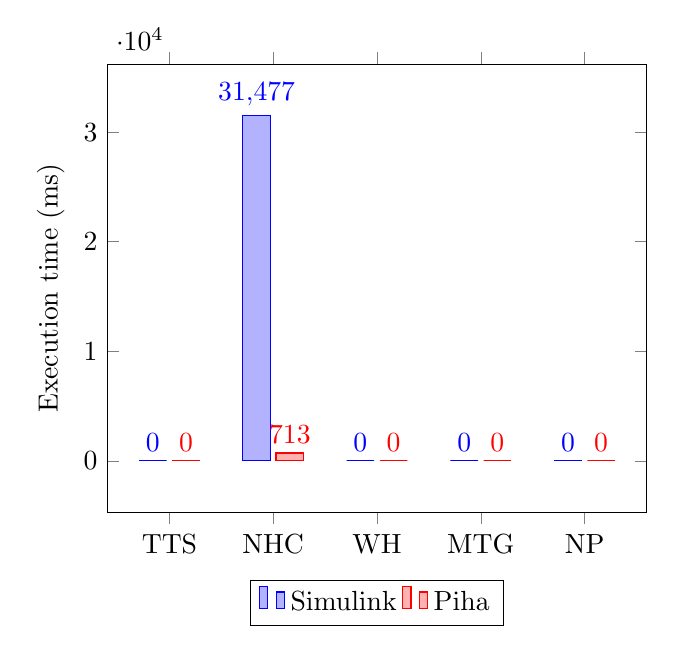
\begin{tikzpicture}
\begin{axis}[
	ybar,
	enlargelimits=0.15,
	legend style={
		at={(0.5,-0.15)},
		anchor=north,
		legend columns=-1
	},
	ylabel={Execution time (ms)},
	symbolic x coords={TTS, NHC, WH, MTG, NP},
	xtick=data,
	nodes near coords,
	nodes near coords align={vertical},
]

%Simulink
\addplot coordinates {
	(TTS,0)
	(NHC,31477)
	(WH,0)
	(MTG,0)
	(NP,0)
};

%Piha
\addplot coordinates {
	(TTS,0)
	(NHC,713)
	(WH,0)
	(MTG,0)
	(NP,0)
};

\legend{Simulink, Piha}

\end{axis}
\end{tikzpicture}

  }
  \subfigure[Executable size (KB) \label{fig:executableSize}]{
    \begin{tikzpicture}
\begin{axis}[
	ybar,
	width=\linewidth-5mm,
	height=5cm,
	enlarge y limits={upper, value=0.1},
	enlarge x limits=0.15,
	legend style={
		at={(0.5,1.15)},
		anchor=north,
		legend columns=-1
	},
	ylabel={Executable Size (KB)},
	ymin=0,
	symbolic x coords={TSN, NHN, WH, MTG, NP},
	xtick=data,
%	nodes near coords,
	nodes near coords align={vertical},
]

%Simulink
\addplot coordinates {
	(TSN,190)
	(NHN,320)
	(WH,226)
	(MTG,188)
	(NP,212)
};

%Piha (O0)
\addplot coordinates {
	(TSN,131)
	(NHN,323)
	(WH,163)
	(MTG,130)
	(NP,174)
};

%Piha (O2)
\addplot coordinates {
	(TSN,96)
	(NHN,128)
	(WH,98)
	(MTG,97)
	(NP,98)
};


\legend{\simulink, \ourTool (O0), \ourTool (O2)}

\end{axis}
\end{tikzpicture}

  }
  \caption{Comparison of the execution time (in ms) and executable size
    (in KB) between \simulink and \ourTool for the benchmarks in
    Table~\ref{tab:benchmarks}.}
  \label{fig:results}
\end{figure}

For the second experiment, we use the five benchmarks
presented in Table~\ref{tab:benchmarks}.  The table also presents the
number of locations (\#L) in each hybrid automata.  For example,
$(2^{50})$ denotes that the \acf{TSN} benchmark is described by $50$~instances 
of an \ac{HIOA} with two locations.

For all the benchmarks, the executable for the \simulink models are
generated using the in-built Real-time
Workshop\textsuperscript{\textregistered} C code generator.  Similarly,
for \ourTool, we generate equivalent C code, and compile it using a
standard C compiler.
The execution times and executable sizes of the generated programs are reported 
below and illustrated in Figure~\ref{fig:results}.

\textbf{Execution time:} Figure~\ref{fig:executionTime} shows that for
all benchmarks the execution time of \ourTool (both without optimisation
and with optimisation level \texttt{O2}) is faster than that of
\simulink.  On average, we show that \ourTool is $9.8$~times faster than
\simulink.
For our most complicated example, the \ac{NHN}, we observe an improvement of 
$20.3$~times.

\textbf{Code size:} Figure~\ref{fig:executableSize} shows that the code
generated by \ourTool is also, generally, more compact than that
generated by \simulink.  On average, the optimised code of \ourTool is
$54\%$ smaller than \simulink when compiled.
For the \ac{NHN} example, the unoptimised code of \ourTool is comparable to 
that of \simulink while the optimised code sees improvements similar to that of 
the other benchmarks.

%In summary, the code generated by \ourTool executes $9.8$~times faster
%on average, with the executable size being $54\%$ smaller on average
%when compared to \simulink.

\begin{table*}
	\centering
	\caption{Benchmark descriptions
	\label{tab:benchmarks}}
\begin{tabular}{ | c | c | c | l | } \hline
\textbf{Benchmarks}
	& \textbf{Domain} 
	& \textbf{\#L } 
	& \textbf{Description} \\ \hline

	\acf{TTS}
		& Physics~\cite{Pedro2005}
		& $(2, 2, 2)$
		& Three thermostats heating a room to keep it warm\\ \hline
		
	\acf{NHC}
		& Biology~\cite{chen201487}
		& $(4^{33})$
		& Captures the electrical conduction system of a heart with $33$ nodes\\ \hline

	\acf{WH}
		& Physics~\cite{raskin05}
		& $(4, 4)$
		& Models the heating of water in a tank \\ \hline
		
	\acf{MTG}  
		& Industrial automation~\cite{Costello2013}
		& $(2, 3^{30})$
		& Models the behaviour of a gate and $30$ trains at a rail road crossing\\ \hline
		
	\acf{NP}
		& Industrial automation~\cite{alur2015book}
		& $(3^{30}, 3^{30})$
		& Switches between two fuel rods in 30 reactors to avoid nuclear meltdown\\ \hline
	
	
 \end{tabular}
 \end{table*}


%%% Local Variables:
%%% mode: latex
%%% TeX-master: "../DATE2016_codegen"
%%% End:

\section{Related work}
\label{sec:lit}
There are many solutions for code generation from \acf{HA}...
\begin{itemize}
	\item Upenn timed automata
	\item Simulink
	\item ....
\end{itemize}
\section{Conclusions}

We propose an approach of modular code generation 
from hybrid input output automata (HIOA)
for the emulation of diverse physical processes. 
We have used the developed approach to model 
 a complex electrical conduction network of a human heart.
% consisting of 
%network of cardiac nodes may 
%be modelled along a conduction pathway of the human heart.
Each node of the network is modelled as a single HIOA.
%such that the voltage of a node is influenced by adjoining nodes.
This composition of nodes is achieved using the concept of 
delayed synchronous composition, similar to the SL 
language~\cite{SlLanguage}. 
This enables the nodes to effectively operate 
in a truly parallel manner as all
input-output dependencies are delayed. 
%Also, we have developed a synchronous semantics of HIOA that enables the mapping of 
%an individual HIOA to a standard synchronous FSM. 
%The key idea is that the synchronous instant or tick is 
%used both as the step size for performing numerical integration
% (when control resides in a location) and also when 
%any transition is taken to a different location. 
The developed approach,  ``compiles away'' the continuous dynamics to
produce pure synchronous code for each node with delayed composition between nodes for creating the behaviour of a large conduction 
pathway with many nodes. Such an approach for modular and scalable code generation from hybrid automata without the reliance on external numerical solvers is new.
\ignore{The developed approach is founded on mathematical semantics and the generated core is guaranteed to
be sound by construction.} 

We compared the developed approach with the commercial tool \simulink. We show that our approach for modular code generation from \ac{HIOA} can 
provide, on average $9.8$ times faster execution and $54\%$ smaller executables 
when compared to \simulink.
We also show that for the \acf{NHN} benchmark our approach is capable of 
emulation of networks that are $5$ times more complex. 
In the future, we will compare our approach quantitatively with Z\'{e}lus~\cite{bourke13zelus},
 which is a synchronous code generator from hybrid automata that relies on dynamic interactions with numerical solvers.
%We will also model re-entrant behaviour in the conduction pathway, unlike the forward conduction system modelled here.

\ignore{While this paper focuses on the example of cardiac pacemakers the proposed code generation for emulation of plant is applicable beyond just the medical domain.
This is illustrated through the diverse range of benchmarks presented in Section~\ref{sec:diversity}.

We show that our approach for modular code generation from \ac{HIOA} can 
provide, on average $9.8$ times faster execution and $54\%$ smaller executables 
when compared to \simulink.
We also show that for the \acf{NHN} benchmark our approach is capable of 
emulation of networks that are $5$ times more complex.

The usage of numerical methods for the solving of \acp{ODE} means our approach is highly dependent on the step size $\delta$ in order for correct emulation.
Thus, the use of higher order \ac{ODE} solvers (such as Runge-Kutta) may need to be investigated in order to allow the step size $\delta$ to be increased.
While our approach requires the \ac{HIOA} from which code is generated to be 
deterministic, the emulation of such non-deterministic \ac{HIOA} is something 
to be investigated.}



\bibliographystyle{ieeetr}
\bibliography{references} 

\end{document}


